
\chapter{CONTRIBUTION 3: Research Questions And The Design Of Pond}
\label{cha:cont3}
 

In this chapter, I describe the design of POND, the Pattern-Oriented Nutrition Diary. In earlier chapters, I described the challenges and barriers that people face when employing a traditional approach to journaling what they eat, either on paper, a website/software, or on a PDA/mobile phone, and then characterized tradeoffs and preferences between traditional food journaling and index-based food journaling on mobile phones. Initial research indicated there could be a benefit for some people and some situations, although the lab-based research is unable to reflect the context and constraints that people encounter in the real world. In this chapter, I refer to the design considerations outlined in the previous chapter, identify specific research aims for evaluation a food index-based food diary in situ, and document the design of a mobile phone food index-based food diary. 

\section{Introduction}
The Pattern-Oriented Nutrition Diary (POND) project is the result of the previous two studies. Participants in the BALANCE study taught us that looking up in the database was a challenge, and from the previous study that people in general preferred the HEI-based food diary to the FBQI-based food diary, due to the quality of information that it captured. 

The goal of POND was to design and build a food diary that incorporated what we learned in the previous studies, and investigate whether experience the findings were applicable in the real world (as opposed to just a lab setting). Feedback from BALANCE participants indicated that they felt BALANCE required too much time and effort to make entries, and that they would be willing to sacrifice detail in exchange for an interface that was quicker and easier to use. The previous comparison study showed that while the FBQI-based interface was quickest and easiest to use, it didn't provide enough value in terms of the data/detail it collected. Participants were divided on whether they preferred the detail-oriented BALANCE interface, or the quicker-yet-still-valuable HEI interface to address their personal eating goals. 

POND was designed to reflect the HEI. Initial user testing showed that people felt too uncomfortable entering the pattern directly for combination or prepared foods, so a food lookup feature was added. This used the NutritionistPro Knowledge Base [ref] food diary (as in the BALANCE and Comparison Study), and was intended to be used as an alternate entry strategy. 

In the rest of this chapter, I first discuss the research questions we were looking to answer, then address some overarching design decisions that impacted the design of POND, and finally focus on the final design of the POND app. 

\section{Research Aims}
The goal of this project was to design and build a food diary that incorporated what we learned in the previous studies, and investigate whether experience the findings were applicable in situ.
\subsection{Primary Research Question: }

Given a food diary that requires less time to use but provides less detail overall, will people use it ``longer''? 

\subsection{Secondary Research Question: }
\begin{itemize}
\item Will the ability to customize the interface to minimize it to the things you care about (``goals'') impact the use of the tool? 
\item If the default interface contains items the users don't really care about, and are just taking more time for entry, do they get rid of them and keep tracking? 
\item Are people willing to minimize the tracking time? 
\item How/when/for what do people use the food database lookup feature? 
\end{itemize}
\section{Overarching Design Considerations}

The instruments designed for the in-lab study comparing BALANCE, HEI and FBQI provided insight as to interface and interaction concerns, as well as ideas for how to make a food index-based food diary more useful. Here, I outline the concerns and suggestions, and identify how they impacted the design of POND. 
\subsection{Potential Challenge: Increasing entry time; combining analysis \& entry on one page;} 

One key design strategy embodied in the HEI and FBQI interfaces was combining record entry and daily analysis mostly on one screen. This differs from the BALANCE interface, which showed an analysis or overview on one screen, and opened a different screen (or series of screens) for creating an entry. Since the goal of the project is to minimize the time and thinking that goes into capturing the food entry, it's important to think this through. 

\subsubsection{Direct Manipulation Versus ``Fill Out A Form'' Entry}
Initial visions (and the in-lab research prototypes) were informed by the design goal of reducing the number of steps to create an entry. One can imagine an extreme end of this, where a visualization shows the current overview for the day, and as one drags a finger/pointer across the visualization, the values change and an entry is recorded. Potential downsides include accidental entries and a greater learning curve. Additionally, the visualization needed to be able to adjust to the goal components and values changing over time. 

An alternate approach is more similar to that used by BALANCE, in which a form pops up and needs to be filled out, item by item, and then the entry confirmed. This approach provides more guidance, but is also more time consuming and likely to be less convenient. 

This was addressed by having each component represented by a widget that included a title, description, feedback, and entry button. The component widgets could then be added to the screen as desired, and the list of widgets could extend past the end of the screen. This approach is reasonable on modern smartphones, since a scrolling interaction is responsive, and expected by users. 

\subsubsection{Quick-Add Versus Add-Earlier-Entry}

While POND is being designed in the hopes that people will use it regularly throughout the day, the fact is that sometimes, people will forget to make an entry. This was not a problem in the BALANCE software, as the add-entry screen included a widget to specify what time the food was eaten. Therefore, there was no difference in process to add a food either for now or earlier, but if a user was adding a food for earlier they would change that value. As mentioned in the previous section, for POND, we wanted to streamline the entry process as much as possible, and that meant not opening another window for creating entries. While this did streamline an entry for now, it required lengthening the process of making an entry for earlier. 

\subsection{Potential Challenge: How to count a food}
The in-lab study showed us that people were uncertain about how to count a food using the food index. To ensure that their self-monitoring was beneficial, participants wanted more guidance on how to break a food into its index components. 

\subsubsection{Looking Up Food Entries}
Initially, the POND prototype included explanations and examples for each of the components. However, initial feedback indicated that people really wanted some more certainty. This appeared to be particularly important when people were just becoming familiar with the counting approach. Therefore, we added a food lookup feature to the POND prototype. The lookup feature does not provide a perfect component profile for each food , due to the limitations of the database, but does provide some guidance. 

\subsection{Potential Challenge: Serving sizes}
Serving sizes were an area of concern in the in-lab comparison study. Concerns included how to figure out how much was eaten, whether to round up or round down when counting a partial serving, and how much of something to count (for example, do I enter the slice of tomato on my salad?).

\subsubsection{Serving Sizes}
We addressed the serving size problem by referring to consumer-oriented literature developed by the USDA to educate consumers about the healthy eating guidelines [ref][USDA2010]. We ensured that the serving size amounts related to a real-world item to compare to. The amounts for the food group items were based on ``typical serving sizes''. For fruits and vegetables, it was � cup, which was explained in terms of common servings (2 blocks is a serving the size of your fist, a small apple, etc); grains was in terms of � cup (baseball, fist) or a slice of bread, pancake the size of a DVD, etc. Partial servings were supported by allowing the user to enter � of a serving. 


\subsection{Potential Challenge: Not knowing if you've entered something or not}

With the HEI and FBQI interfaces, observations of and feedback from participants in the in-lab study revealed occasional confusion over whether a food item was entered or not. 
\subsubsection{Time- And Location-Based Analysis}
To address this problem we considered how we can automatically capture some context about the entry, and use that to help people decide if they entered either something they just ate, or something from a few hours ago. Entries can be tagged time and location automatically. We designed the interface to support tracking entries with user-defined locations. For times when the location can't be detected, all known (user-defined) locations can be easily chosen from a drop-down list on the front screen. 

\subsubsection{Grouping Entries}
Another way we attempted to provide feedback about what entries have been made is to group entries together via time. Entries made within a certain amount of time (for the in situ evaluation, it was set at 45 seconds) were grouped together, and shown on the ``daily history'' list together, as opposed to separately. This is discussed in further detail later. 

\subsubsection{Shortcuts/Combos}

Finally, we designed a ``favorites'' feature. This allowed users to define an entry themselves. A combination consists of a name (such as ``Turkey Sandwich''), and the components that create it (2 whole grains, 3 proteins, 1 dairy, 1 sat fat, 3 sodium). When this is used for an entry, the name of the food is shown in the daily history list, which is described further later. 
\section{Design}
The primary goal informing the design of the POND app was to minimize the amount of time it took to make an entry. 

\subsection{Home Screen/Launch Activity}
The first screen the user sees when they launch POND is the home screen, shown in Figure 1. This screen was designed to prioritize quick entry and quick analysis of the current progress towards goals for the day. Each row represents a recommendation from the 12 USDA Dietary Guidelines we have described above. Users can touch the +1 buttons on the right side of the screen to quickly indicate a portion eaten, or long-press the +1 buttons to indicate a � portion eaten. Colored links expand to show information about what counts in a given component (item), or what makes a serving. This information was adapted from the USDA 2010 Dietary Guidelines. 

Location is indicated in a drop-down menu across the top. It automatically tries to determine which pre-defined location the user is in (Home, Work) or ``Other'' if it is an unfamiliar location, and the blue ``+'' button opens the ``Add Food'' Screen. The phone's search button can also be used to launch a search widget and search for a given food. 

\begin{figure}	
	\centering
	\begin{subfigure}[t]{1.25in}
		\centering
		\setlength\fboxsep{0pt}
\setlength\fboxrule{0.5pt}
\fbox{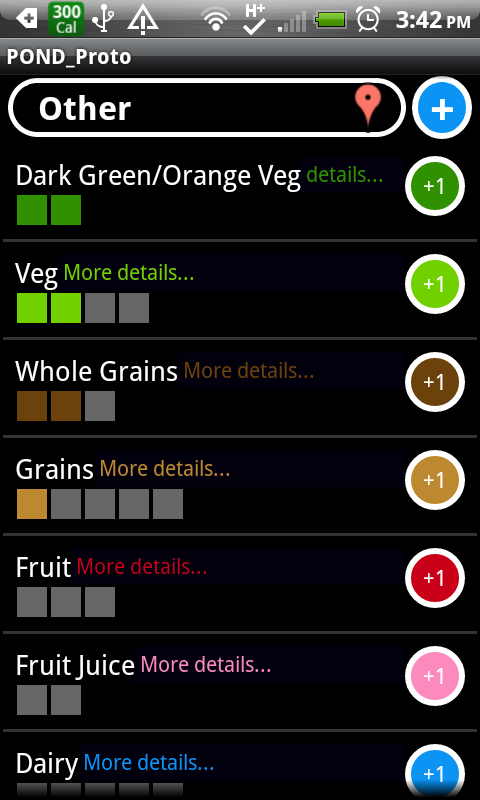
\includegraphics[width=1.25in]{./images/cont3/fig1a}}
		\caption{To make a new food entry, select the `Add Food' menu item. }\label{fig:fig3_1a}
	\end{subfigure}
\quad
\begin{subfigure}[t]{1.25in}
		\centering
		\setlength\fboxsep{0pt}
\setlength\fboxrule{0.5pt}
\fbox{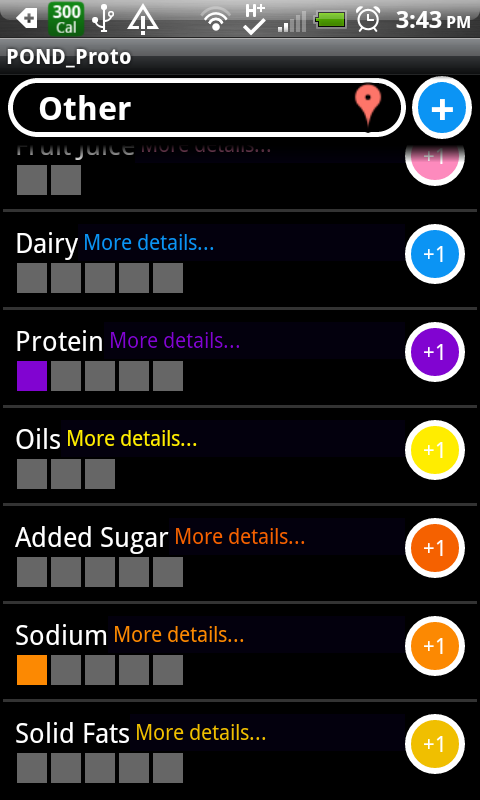
\includegraphics[width=1.25in]{./images/cont3/fig1b}}
		\caption{Enter the food name. }\label{fig:fig3_1b}
	\end{subfigure}
\quad
\begin{subfigure}[t]{1.25in}
		\centering
		\setlength\fboxsep{0pt}
\setlength\fboxrule{0.5pt}
\fbox{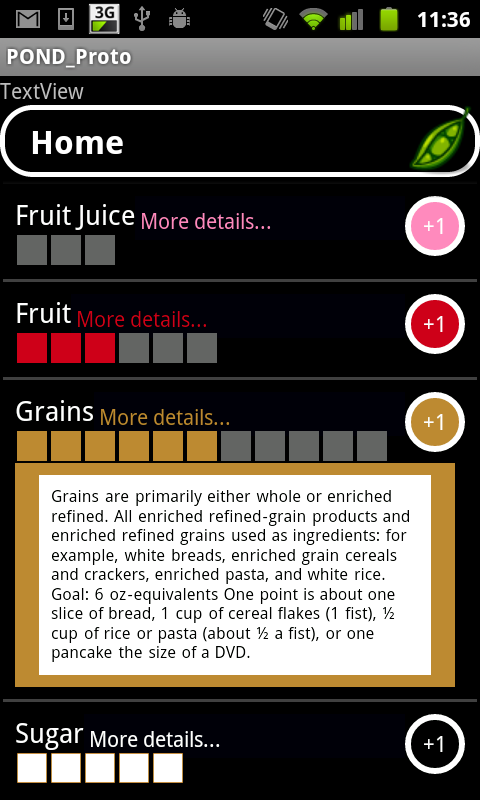
\includegraphics[width=1.25in]{./images/cont3/fig1c}}
		\caption{When the food name has not been used before, the user is given the option to either bookmark the entry to fill out later, create a manual entry using the nutrition facts label now, or query the database.}\label{fig:fig3_1c}
	\end{subfigure}
\quad
\begin{subfigure}[t]{1.25in}
		\centering
		\setlength\fboxsep{0pt}
\setlength\fboxrule{0.5pt}
\fbox{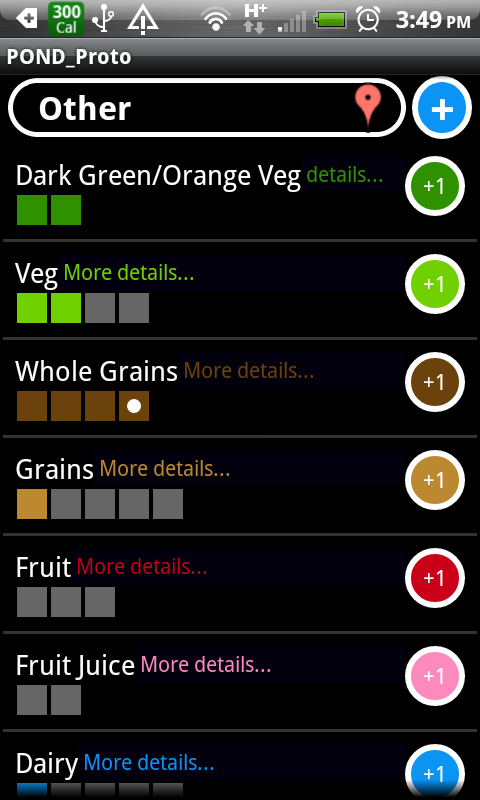
\includegraphics[width=1.25in]{./images/cont3/fig1d}}
		\caption{When there are many entries, the user is asked to choos a food group to filter the results. }\label{fig:fig3_1d}
	\end{subfigure}

	\caption{POND Screens}\label{fig:fig3_1}
\end{figure}


For the components, dark gray boxes indicate the current daily goal for that component. A colored box indicates how many portions of that component have been consumed. A colored block with a white dot indicates that the user has consumed more than the goal number of blocks. The use of a white dot in the block was chosen in order to provide non-judgmental feedback about the amount of servings consumed. 

\subsection{Daily Entries}
The ``Daily Entries'' screen was designed to show a list of the entries made over time so far today. The entries are reversed-ordered, with the most recent entry at the top. Here, users can distinguish between which items were looked up in the database versus which items were added with a +1. +1 Entries made very close together in time (~15 seconds) are grouped together into one item, as they are usually connected. The entry is also tagged with the location. 
The purple + button allows users to go directly to the ``Add Food'' Screen, while the device search button opens up a search widget to allow the user to add a new item to the showing day's list. Different days can be viewed by using the arrow buttons at the top of the screen, or by swiping left/right. Touching one of the entries opens up the appropriate ``Entry Edit'' screen and allows just that entry to be edited. A long touch on one entry shows a menu which allows the chosen single entry to be either edited or deleted. 

\begin{figure}	
\centering
	\begin{subfigure}[t]{1.25in}
		\centering
		\setlength\fboxsep{0pt}
\setlength\fboxrule{0.5pt}
\fbox{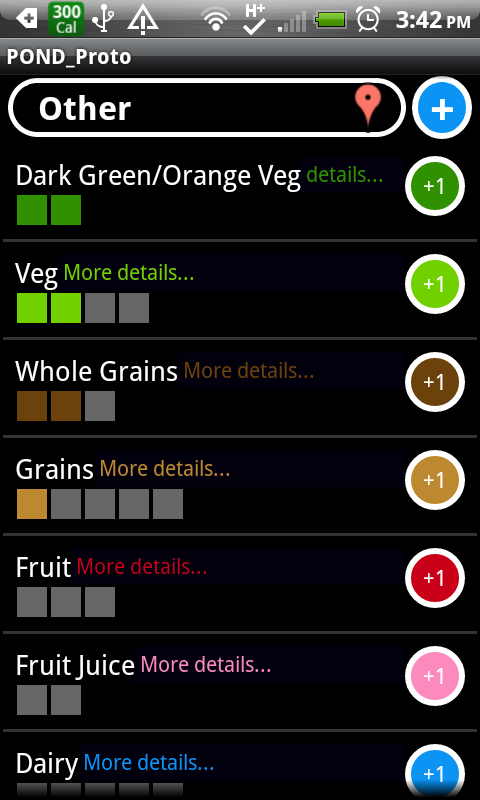
\includegraphics[width=1.25in]{./images/cont3/fig1a}}
		\caption{To make a new food entry, select the `Add Food' menu item. }\label{fig:fig3_1a}
	\end{subfigure}
\quad
\begin{subfigure}[t]{1.25in}
		\centering
		\setlength\fboxsep{0pt}
\setlength\fboxrule{0.5pt}
\fbox{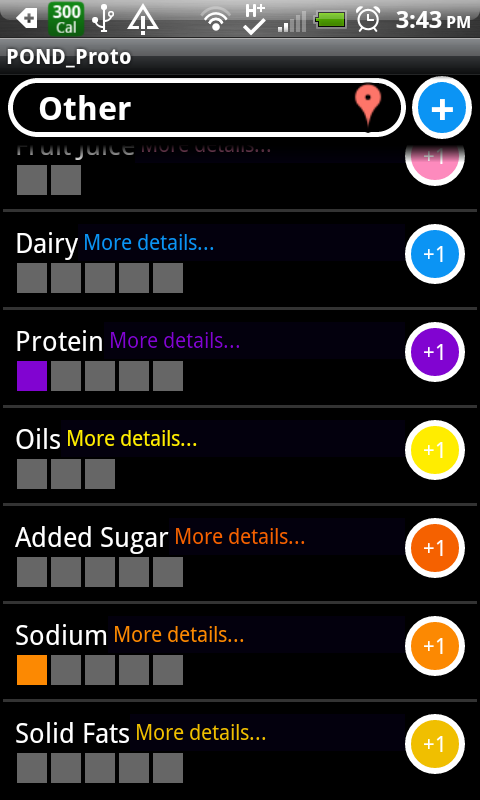
\includegraphics[width=1.25in]{./images/cont3/fig1b}}
		\caption{Enter the food name. }\label{fig:fig3_1b}
	\end{subfigure}
\quad
\begin{subfigure}[t]{1.25in}
		\centering
		\setlength\fboxsep{0pt}
\setlength\fboxrule{0.5pt}
\fbox{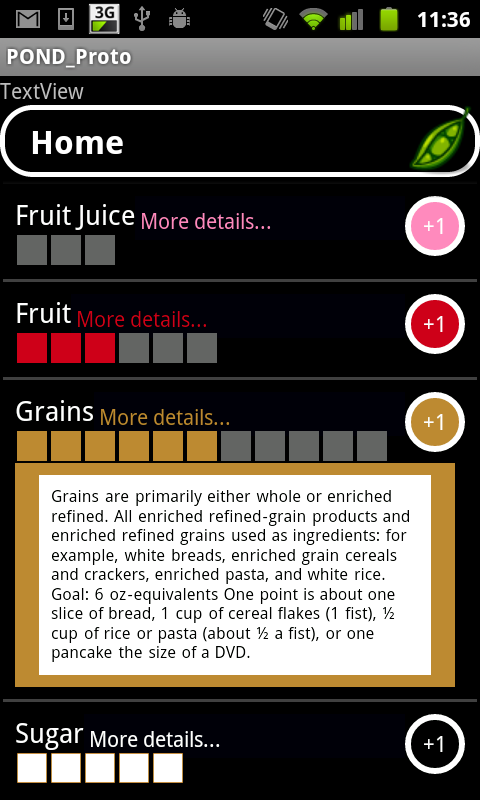
\includegraphics[width=1.25in]{./images/cont3/fig1c}}
		\caption{When the food name has not been used before, the user is given the option to either bookmark the entry to fill out later, create a manual entry using the nutrition facts label now, or query the database.}\label{fig:fig3_1c}
	\end{subfigure}
	\caption{POND Screens.}\label{fig:3_1}
\end{figure}

\subsection{Create Custom, Frequently-Eaten Foods}
This screen supports the creation of shortcuts for food combinations that people frequently eat. Note, this is just a combination of ``+1''s; not a combination of foods from the database, and it's intended to be a single serving (or, amount eaten at one time), as opposed to a recipe, which one might eat multiple or varying servings of. The example in the screenshot is a turkey sandwich: it's composed of two whole grains (for the bread), and if you scroll further down, some meat, some dairy, some solid fat for the cheese, some oil for the mayo, and some sodium for the bread, meat, and cheese. When the user then eats this turkey sandwich again, they can find it in the list of ``My Foods'' (description coming), and quickly enter it. The given, personalized name (``My Turkey Sandwich'') is then shown in the list of entries made today as a named group of blocks. The ``Add to Diary'' button allows the user to create a new entry for both current and future use, while when the ``Add to Diary'' checkbox is not checked, it just saves it for future use. 

\begin{figure}	
\centering
	\begin{subfigure}[t]{1.25in}
		\centering
		\setlength\fboxsep{0pt}
\setlength\fboxrule{0.5pt}
\fbox{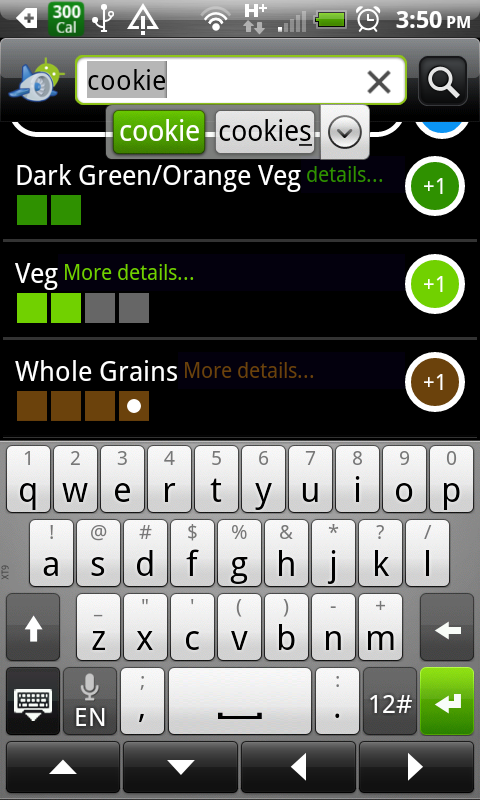
\includegraphics[width=1.25in]{./images/cont3/fig3a}}
		\caption{To make a new food entry, select the `Add Food' menu item. }\label{fig:fig3_1a}
	\end{subfigure}
\quad
\begin{subfigure}[t]{1.25in}
		\centering
		\setlength\fboxsep{0pt}
\setlength\fboxrule{0.5pt}
\fbox{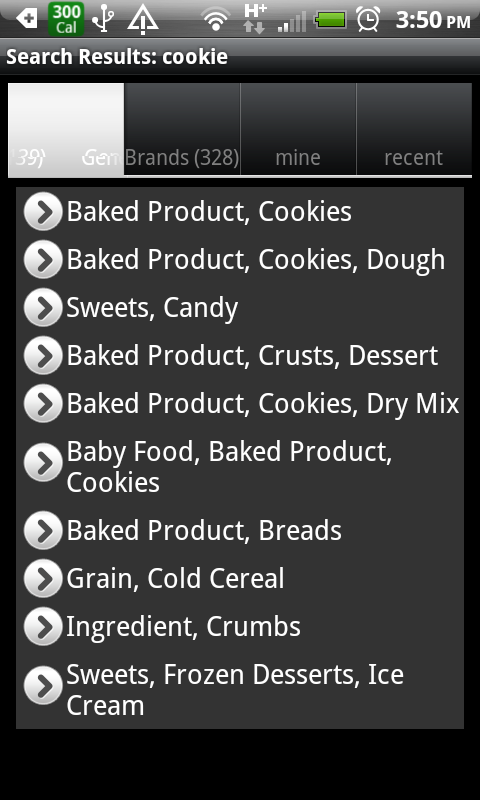
\includegraphics[width=1.25in]{./images/cont3/fig3b}}
		\caption{Enter the food name. }\label{fig:fig3_1b}
	\end{subfigure}
\quad
\begin{subfigure}[t]{1.25in}
		\centering
		\setlength\fboxsep{0pt}
\setlength\fboxrule{0.5pt}
\fbox{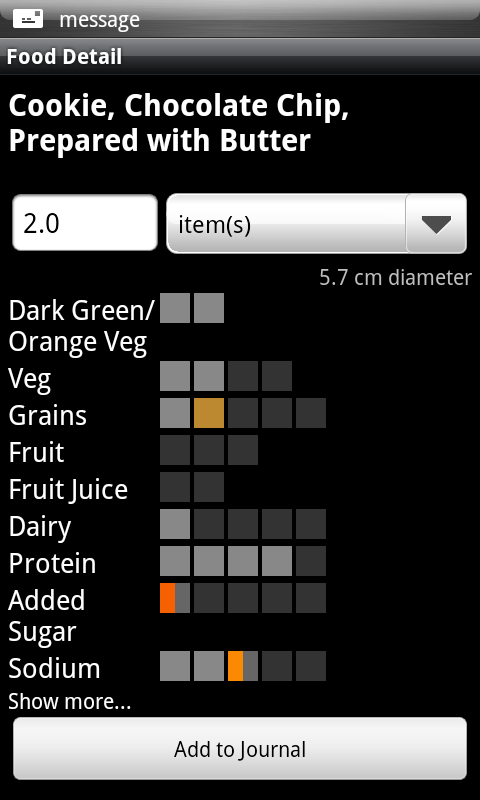
\includegraphics[width=1.25in]{./images/cont3/fig3c}}
		\caption{When the food name has not been used before, the user is given the option to either bookmark the entry to fill out later, create a manual entry using the nutrition facts label now, or query the database.}\label{fig:fig3_1c}
	\end{subfigure}
	\caption{POND Screens.}\label{fig:3_1}
\end{figure}



\subsection{Change Goals Screen}
The change goals screen can be used to change which components appear on the front screen, as well as how many blocks appear for each component. The checkboxes on the right are checked ``on'' to appear on the front screen, and the +/- buttons are used to indicate how many blocks should be provided for each component. Default USDA suggestions are indicated. When the number of blocks for an item is less than the suggested number of blocks for a component, light gray blocks indicate how many more are needed to get to that amount. When more blocks are selected than the suggestion, the blocks have a white circle inside. 


\begin{figure}[ t ]
\centering
\setlength\fboxsep{0pt}
\setlength\fboxrule{0.5pt}
\fbox{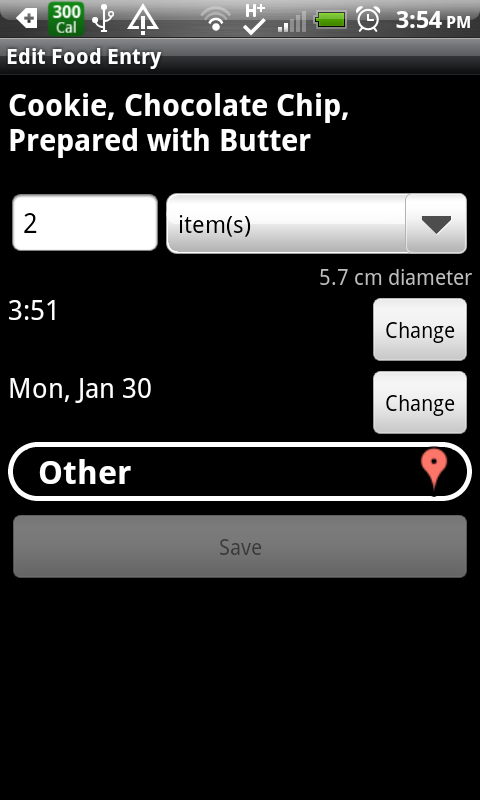
\includegraphics[ width =2.5cm ]{./images/cont3/fig4a}}
\label{fig:fig3_4a}

\caption{POND Screens.}
\end{figure}

\subsection{Search process/screens}
Food from the database or custom created foods can be added from either a search or chosen from a list of foods used before. The device search button can be used to launch the search widget from either the home screen or the daily entries screen. The search term is used for a full-text search in the food name and manufacturer fields of the database. The results are broken into ``Generic'' and ``Brand'' tabs (as designated by the database). Within each grouping, if there are fewer than 100(?) results, the results are presented alphabetically. If there are more results, the results are presented in a two-level list, grouped by ``Food Class'', as designated by the database, with the food classes ordered such that the class with the most entries is at the top of the screen, and alphabetically within the food class. From this page, the user can either ``Refine'' the search, or start a new search. 

The other two tabs on this ``Chose Food'' screen include only foods that have been used before or have been created by the user. The ``Mine'' tab lists foods alphabetically, while the ``Recent'' tab lists the same foods by the order they were last used, most recent on top. 

Once a food has been found and selected, the Food Detail screen shows more information about that food. It allows the user to change the serving size amount. The screen also displays how eating the specified amount of the chosen food will impact the goals for the day if eaten. The dark gray blocks represent the goal for that component, while the light gray blocks show what has already been consumed today. The colored boxes show the components due to the chosen food. 

\subsection{Editing Entries}

There are two different Entry Edit screens: one for Food entries (from the database), and one for +1 or custom food entries (which are treated like a combination of +1 entries). For food entries, the user can pretty much just change the amount, time, date, and location of the item. For +1 or custom food entries, the user can edit the name (or give it a new, meaningful name) and add/edit/delete the components, as well as change the time, date and location of the entry. 
\subsection{Weekly Feedback}

The weekly summary screen provides feedback about progress towards the goals throughout the week. The blue bars show the daily goal, or what that goal was for that day, empty boxes show that a goal hasn't been reached, while boxes extending past the bar show a goal that has been passed. Each screen only shows one component, and the drop-down list at the top (or swiping up/down on the screen) changes the component being displayed. Different weeks can be chosen via the menu, or swiping left/right on the screen. 

\begin{figure}	
\centering
	\begin{subfigure}[t]{1.25in}
		\centering
		\setlength\fboxsep{0pt}
\setlength\fboxrule{0.5pt}
\fbox{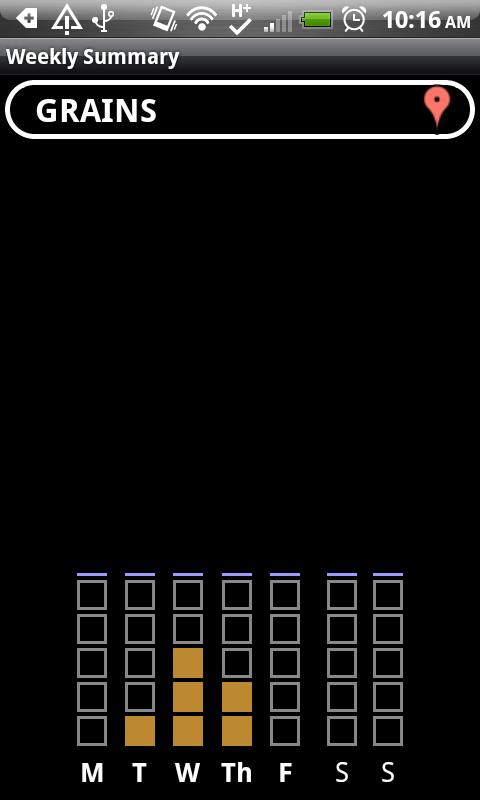
\includegraphics[width=1.25in]{./images/cont3/fig5a}}
		\caption{To make a new food entry, select the `Add Food' menu item. }\label{fig:fig5_1a}
	\end{subfigure}
\quad
\begin{subfigure}[t]{1.25in}
		\centering
		\setlength\fboxsep{0pt}
\setlength\fboxrule{0.5pt}
\fbox{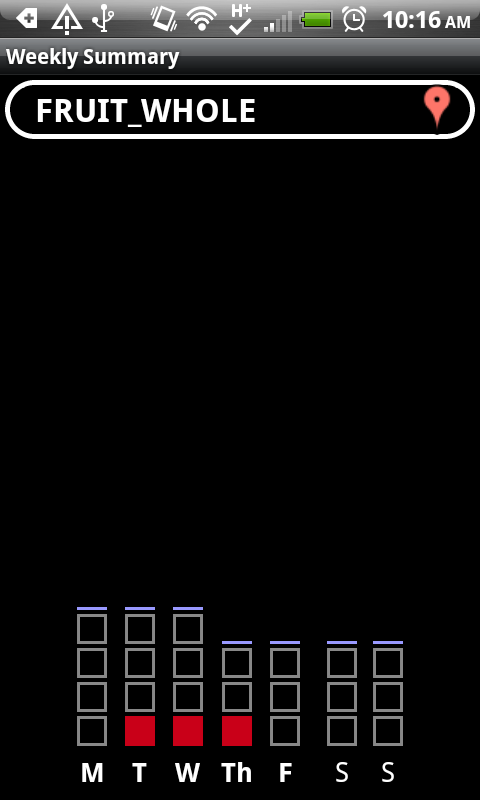
\includegraphics[width=1.25in]{./images/cont3/fig5b}}
		\caption{Enter the food name. }\label{fig:fig5_1b}
	\end{subfigure}
\quad
\begin{subfigure}[t]{1.25in}
		\centering
		\setlength\fboxsep{0pt}
\setlength\fboxrule{0.5pt}
\fbox{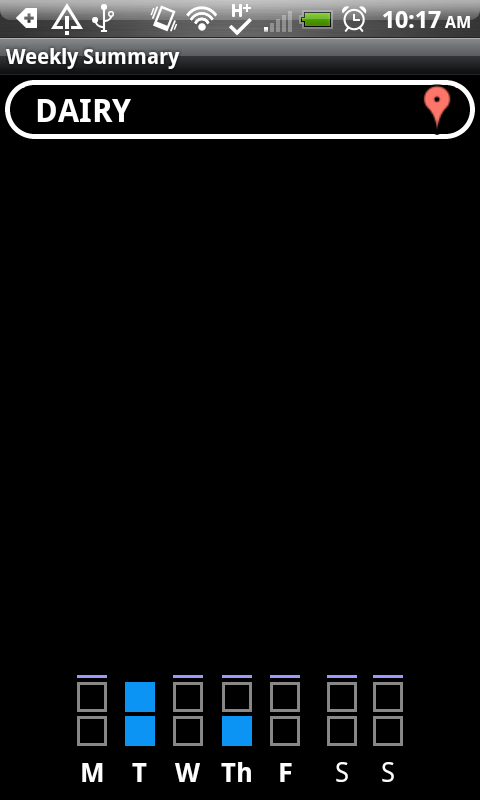
\includegraphics[width=1.25in]{./images/cont3/fig5c}}
		\caption{When the food name has not been us.}\label{fig:fig5_1c}
	\end{subfigure}
	\caption{POND Screens.}\label{fig:3_1}
\end{figure}



\section{Summary}

In this chapter, I provided a detailed description of the POND food diary. The POND food diary was designed to require minimal resources in terms of time and decision making to capture dietary intake information. The design of POND was informed by user feedback and studies discussed earlier in this dissertation. POND was designed to represent the HEI, which received favorable feedback in earlier studies, and informed by information from the USDA's Healthy Eating Guidelines. The design of a food lookup feature was informed by experiences with the BALANCE studies. Reflections on the design are discussed in more detail in the next chapter. 
